% ------------------------------------------------
%          FILE:  introducao.tex
%       CREATED:  Dom 30/Dez/2012 hs 15:57
%   LAST CHANGE:  2013 Apr 03 01:03:23 PM
%        AUTHOR:  Sérgio Luiz Araújo Silva
%          SITE:  http://vivaotux.blogspot.com
%       TWITTER:  @voyeg3r
%         SKYPE:  sergioaraujosilva
% -------------------------------------------------

\chapter{Introdução}\label{cha:intro}

% O comando \label{nome} define o marcador da parte especificada.
% Você pode citar esta seção usando o comando \ref{nome}.

Este livro contendo \pageref{LastPage} páginas é um convite ao auto
aprendizado, uma vez que ele cita dezenas de sites na Internet sendo um guia
para o seu trabalho individual de buscar conhecimento, colocamos aqui algumas
experiências com o intuito de lhe poupar esforço.  Compartilhe este material
com outras pessoas.

Ao longo deste livro você conhecerá uma série de técnicas
e dicas que tem como meta fazer com que você aprenda inglês
de forma mais rápida. Há mais de dois anos venho estudando
inglês e tenho conseguido excepcionais resultados. A soma
de toda essa experiência me levou a compartilhar as minhas
descobertas, tudo de bom que descobri estará aqui para
o deleite dos que tem o desejo sincero não apenas de
aprender Inglês, mas qualquer idioma.

\vspace{0.3\baselineskip}
\noindent
{\footnotesize \ding{42} Durante a leitura você verá vários trechos ou frases
em inglês, isso é proposital, você deverá copiar estas frases e
encontrar a tradução, isso é uma amostra de o quanto você vai
ganhar aprendendo mais inglês!}

\section{O primeiro passo}\label{sec:mil-palavras}

Dominar as palavras mais comuns de qualquer idioma é o principal fundamento,
pois com o domínio das mesmas você será capaz de rapidamente
abandonar o português e assistir vídeos com som e legendas totalmente em
inglês, obviamente que nosso objetivo final é que sejamos capazes de apenas
ouvir um falante nativo e poder entender 100\% do que foi falado.  O livro das
1000 palavras \index{Rubens Queiroz Almeida!1000 palavras} mais comuns da
lingua inglesa, de \index{Rubens Queiroz Almeida} {\em Rubens Queiroz
Almeida}\footnote{queiroz@iname.com}, foi criado à partir do
\index{Projeto Gutemberg} \href{http://www.gutenberg.org/}{{\em Projeto Gutemberg}}%
\footnote{http://www.gutenberg.org/} que digitalizou mais de
1600 livros que já estavam sob domínio público à época, este enorme acervo foi submetido
a um algoritmo\footnote{Programa de computador} que determinou quais são
as palavras mais comuns. Você pode baixar o livro das 1000 palavras mais
comuns do inglês neste link \href{http://goo.gl/jbyBZ}{http://goo.gl/jbyBZ} - Uma vez baixado o livro
você deverá ler as páginas introdutórias que explicam em detalhes
o objetivo do livro, em seguida você irá para o conteúdo propriamente
dito, à partir deste ponto você deve ler uma, duas ou mais páginas todo
dia, e assim você verá o seu vocabulário crescer em pouco tempo de forma
natural.

\vspace{0.3\baselineskip}
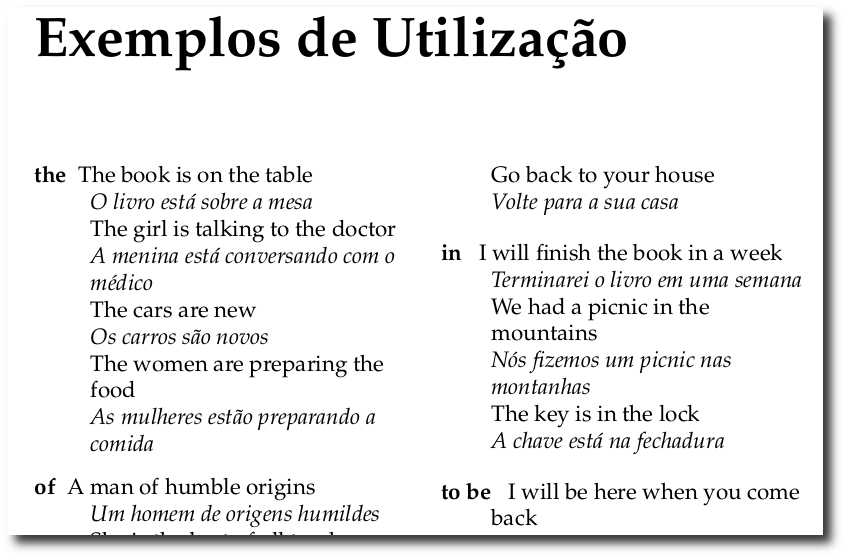
\includegraphics[width=0.8\textwidth]{1000-palavras}

\section{Técnicas Comprovadas por Pesquisas}

Citaremos ao longo do livro pesquisadores na área do ensino de idiomas que fizeram
descobertas que estão mudando a forma como as pessoas aprendem idiomas ao redor
do mundo.

\noindent
\vspace{0.8\baselineskip}
{\scriptsize \ding{42} ``Tell me and I forget, teach me and I may remember, involve me and I learn.'' -- Benjamin Franklin }

\subsection{Busque o nível adequado}

\noindent {\footnotesize \ding{42}
\href{https://blogdopedrojunior.wordpress.com/2010/05/08/estrategias-simples-para-expandir-o-seu-vocabulario-pt-1/}{Referência:
Aprenda inglês fácil.}}

\vspace{0.3\baselineskip} \noindent Você aprende muito mais rápido concentrando-se em
materiais que sejam de fácil entendimento. Esse é um dos pilares do método
desenvolvido pelo especialista em aprendizagem de idiomas, \index{Dr. Stephen
Krashen}
\href{http://adultesljobs.com/dr-stephen-krashen-on-language-acquisition/}{{\em
Dr Stephen
Krashen}}\footnote{http://adultesljobs.com/dr-stephen-krashen-on-language-acquisition/}.
Muitos acreditam que se aprende mais, estudando um material difícil de
entender.  De acordo com as pesquisas do {\em Dr. Krashen}, esse jeito não só
é menos eficiente, como também diminui a motivação do estudante.  Se
a quantidade de palavras não compreendidas for muito alta você ficará
naturalmente desestimulado, portanto busque materiais adequados ao seu nível. A única exceção é se você conseguir por exemplo livros bilingues, nos quais aparecem textos em duas línguas lado a lado, o que facilita a leitura. \\

\noindent
\vspace{0.3\baselineskip}
{\footnotesize \ding{42} Veja também a seção \ref{sec:estrategia} página~\pageref{sec:estrategia}.}

\noindent
{\footnotesize \ding{42} Leia também um artigo sobre o método do Dr.  Stephen Krashen neste
 \href{http://www.readability.com/articles/vdzq7x1o}{http://goo.gl/WCQIc}}

\subsection{Não estude gramática como foco principal}

Segundo estudos de pesquisadores como do \index{Dr. Marvin Brown}
\href{http://www.power-english.net/tag/j-marvin-brown}{{\em Dr. Marvin
Brown}}\footnote{http://www.power-english.net/tag/j-marvin-brown} que
desenvolveu o método \index{Dr. Marvin Brown!Listening Approach} ``The
Listening Approach'', o estudo da gramática na verdade atrapalha o aprendizado,
lembre-se que as crianças quando aprendem a falar apenas ouvem por dois anos ou
mais.  A menos que você seja professor de português eu diria que você não
lembra sequer 1/4 das regras gramaticais que você aprendeu na
escola, no entanto você consegue se expressar bem e também perceber quando
alguém comete um erro de português!

\subsection{Motivos para não estudar gramática}\label{sub:not-grammar}
\index{Gramática}

Você não necessita conhecer os detalhes técnicos de um idioma para usa-lo,
do memo modo que não precisa entender o funcionamento interno de um motor para dirigir
um carro, ou ainda não necessita saber como um processador de computador funciona
para navegar na internet.

Crianças de 4 anos falam sua lingua materna sem saber um vírgula sequer sobre
gramática, se seus pais falam errado elas também falam errado, se seus pais
falam corretamente elas também falam corretamente. Juntando o que aprendemos
sobre o fato de as crianças aprenderem a falar um idioma apenas pelo convívio
podemos somar a isso a ação consciente de anotar sempre as frases inteiras, nas
quais estarão implícitas todas as regras gramaticais. Há ainda outra vantagem
em anotar as frases inteiras, com o tempo você perceberá que sua capacidade de
inferir\footnote{Deduzir o sentido das palavras pelo contexto} o sentido
das palavras pelo contexto irá melhorar substancialmente.

\vspace{0.3\baselineskip}
\noindent
{\footnotesize \ding{42}  Veja como estudar inglês de forma indireta na seção~\ref{sec:EnglishLife}
página~\pageref{sec:EnglishLife}}

\vspace{0.3\baselineskip}
\noindent
{\footnotesize \ding{42}  ``Don't say people you are learning English, just
talk to them about a topic you are interested in \dots ``}

% colocar o link sobre o listening approach
\subsection{Aprenda contextualmente}\label{sub:aprenda-contextualmente}
\index{Aprenda contextualmente}

Quando você se deparar com uma nova palavra não anote apenas a palavra, anote
a frase em que ela se encontra, assim você estará aprendendo a gramática pelo
contexto, ou seja, seu cérebro vai aprender a gramática sem que isso seja uma
preocupação explícita, portanto siga essas duas dicas:

\begin{itemize}
     \item{Não anote palavras isoladas}
     \item{Não estude gramática}
\end{itemize}

\noindent
Entre as muitas vantagens de se estudar frases inteiras citamos o aprendizado
de vocabulário comum a situações específicas veja o exemplo:

\begin{figure}[h!]
	\centering
	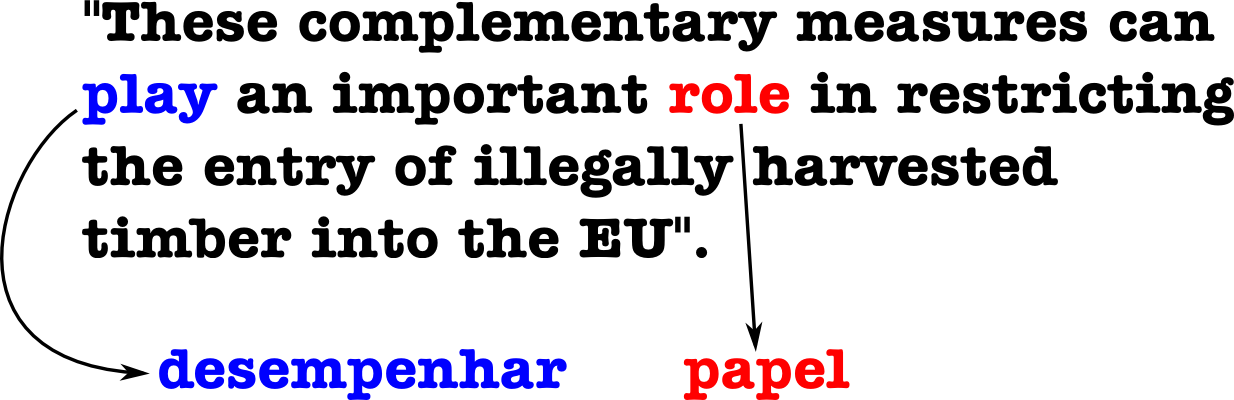
\includegraphics[width=0.8\textwidth]{play-role}
	\caption{play-role}
\end{figure}

\index{Aprenda contextualmente!Linguee} Uma forma interessante de aprender
novas palavras dentro do contexto é através do site linguee
\href{http://www.linguee.pt/}{http://www.linguee.pt/}, nele você escolhe
o idioma de entrada e o de saída e recebe vários textos de exemplo com
a palavra buscada.

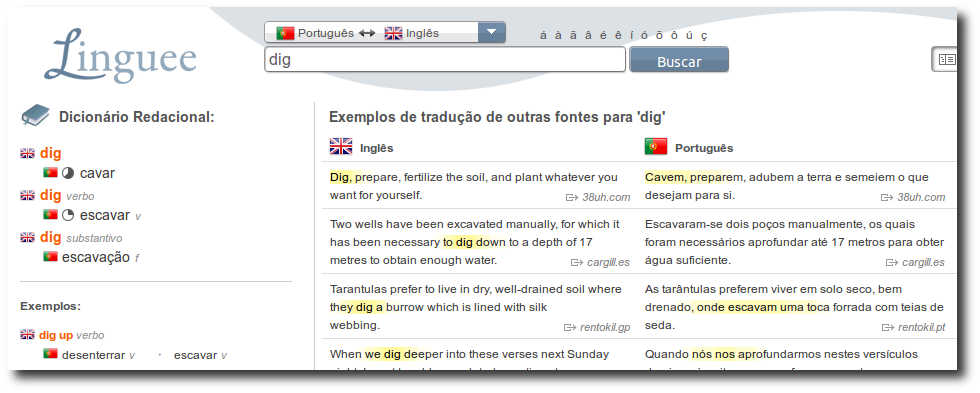
\includegraphics[width=\textwidth]{linguee-exemplos}

\noindent
{\footnotesize \ding{42} Um bom dicionário com exemplos pode ser acessado neste link \href{http://www.yourdictionary.com/}{http://www.yourdictionary.com/} }

\noindent
Outro site muito bom para expandir o vocabulário de {\bf estudantes avançados} é o site
\href{http://www.vocabulary.com}{http://www.vocabulary.com}, com muitos desafios.
\index{Vocabulario}

\begin{figure}[h!]
	\centering
	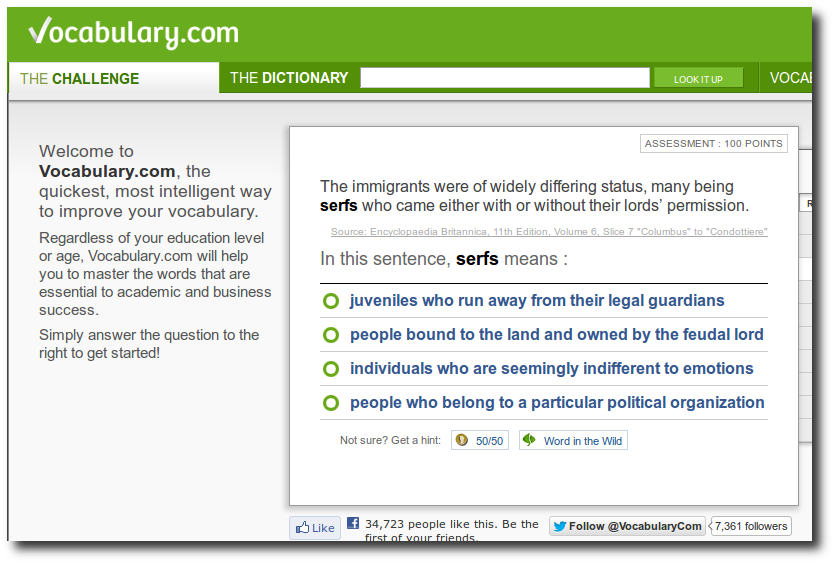
\includegraphics[width=0.8\textwidth]{vocabulary-one}
\end{figure}

% \begin{figure}[h!]
% 	\centering
% 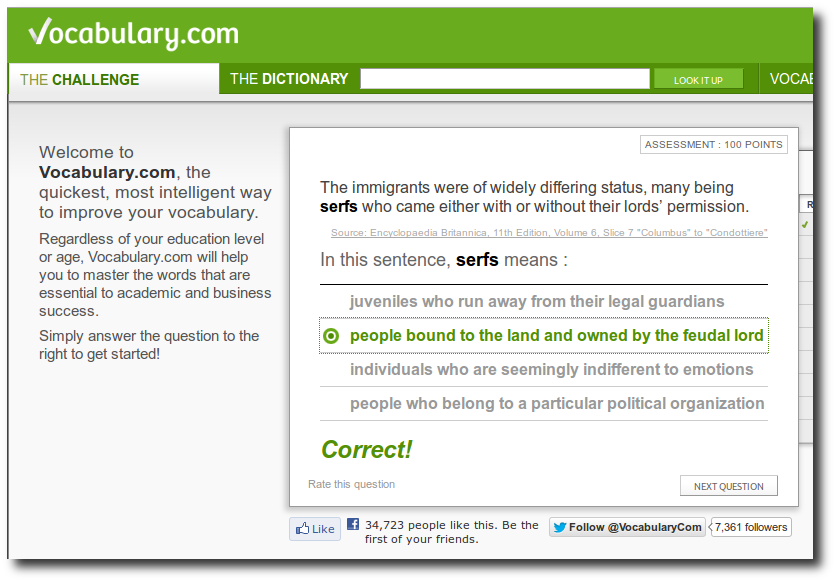
\includegraphics[width=12cm]{vocabulary-two}
% \end{figure}

\noindent
\vspace{0.3\baselineskip}
{\footnotesize \ding{42}  ``English {\em students} learn to pronounce words {\em individually},
and that's why they don't understand native speakers in conversations.''}

\vspace{0.3\baselineskip}
\noindent
{\footnotesize \ding{42} Veja como ter uma espécie de livro de anotações online
na seção~\ref{sec:evernote} página~\pageref{sec:evernote}}

\subsubsection{Leia textos bilíngues}
\label{ssub:leia_textos_bil_ngues}

\begin{multicols}{2}

\noindent
If you work daily with bilingual texts your capacity of understand the
meaning of phrases will rise alarmingly. This exercise will be so
natural to your brain that one day you will notice yourself reading
complicated texts withou any effort.

\noindent
This sort of activity puts you
in a kind of imersion and at same time gives you real context in wich
you will have access rapidly to the translated version, all this make
you acquire the needed skills you must absorb to improve your level faster.

\columnbreak

\noindent
Se você trabalha diariamente com textos bilíngües sua capacidade de
compreender o significado de frases vão subir de forma alarmante. Este
exercício será tão natural para o seu cérebro que um dia você vai
notar-se ler textos complicados withou qualquer esforço.

\vspace{0.5cm}
\noindent
Esse tipo de atividade coloca em uma espécie de imersão e ao mesmo tempo dá-lhe
contexto real no qual você terá acesso rápido para a versão traduzida,
tudo isso faz você adquirir as habilidades necessárias que você
precisa absorver para melhorar o seu nível mais rápido.

\end{multicols}

\pagebreak

\begin{multicols}{2}

During the elaboration this book, more precisely these two columns I
was writing directly the text in Google Translator and copying the
result to this section. In this moments my brain was accessing my
memories to convey you all ideas I needed to you understand this idea.

\vfill \columnbreak

Durante a elaboração deste livro, mais precisamente essas duas colunas eu estava escrevendo
diretamente o texto no Google Tradutor e copiar o resultado para esta
seção. Neste momento o meu cérebro estava acessando minhas memórias
para transmitir-lhe todas as idéias que eu precisava para você
entender esta idéia.

\end{multicols}

% subsubsection leia_textos_bil_ngues (end)


\subsection{Fale sem pensar, fale automaticamente}

Se você estudar muito gramática, toda vez que for falar você tenderá
a traduzir, pensar de forma consciente sobre a gramática, encontrar uma
resposta, traduzir novamente para o inglês, instante no qual a conversa ficará
truncada e anti-natural. Obviamente se você nunca conseguir fazer a sua
conversação fluir um pouquinho que seja, sua confiança também vai pro espaço.

\subsubsection{Lições de conversação}
\label{ssub:li_es_de_conversa_o}

Na verdade a gramática é importante, mas ela não o ajudará a entender
a conversação do dia-a-dia ou a falar inglês naturalmente e
fluentemente sem se sentir embarassado. O único caminho para tornar-se
um falante efetivo em inglês é praticando ouvir e falar tanto quanto
possível. Este trecho foi retirado do site
\href{http://www.englishwithjo.com/english-conversation-lessons/}{http://www.englishwithjo.com/english-conversation-lessons/}
e essas considerações fazem muito sentido, não acha?

Para criar esse tipo de interação você pode criar \emph{Flashcards}
(veja mais sobre os Flashcards na seção~\ref{sub:programas_para_memoria_o} página\pageref{sub:programas_para_memoria_o}) contendo perguntas
cotidianas, de um lado a pergunta em inglês, do outro a resposta. Com
o tempo você vai reformulando os cartões para criar respostas mais
elaboradas. Lembre-se de ler as perguntas e respostas em voz alta para
praticar o listening e a pronúncia.

{\footnotesize \ding{42} Ao ler em voz alta ativamos o lóbulo frontal
do cérebro, que entre outras coisas é responsável pela linguágem.}

% subsubsection li_es_de_conversa_o (end)


\subsection{Repetição}

O nosso cérebro necessita de muitas repetições para gravar novos conhecimentos,
portanto não tenha tanta ânsia por novas lições, uma lição simples mas
explorada de várias formas tais como, fazendo a tradução do texto para
o português, gravando sua voz à partir do conteúdo do texto, a audição do mesmo
material, a transcrição do audio etc.  farão com que seu cérebro assimile mais
rapidamente o conteúdo. A ideia é esgotar todas as possibilidade de aprendizado
em cada lição. Certa vez foi perguntado ao \index{Michael Jordan} {\em Michael
Jordan}\footnote{Talvez o maior jogador de basquete da história} como ele se
tornara um jogador fora do comum, ele respondeu dizendo: ``fundamento,
fundamento, fundamento'', ou seja, ele disse que considerava o estudo dos
fundamentos como sendo o mais importante para se tornar um bom jogador.

Outro aspecto a ser considerado é com relação ao intervalo das
repetições, 10 repetições de 1 minuto em intervalos regulares é mais
eficaz que duas horas ininterruptas de estudo, pois o cérebro vai
cansando e pelo fato de não haver futuras repetições o cérebro tenderá
a descartar essa informação. \emph{Veja mais adiante no texto sobre a
curva de esquecimento}.

Veja como determinação e uso da repetição são bases fundamentais para
o aprimoramento e excelência: \index{Airton Senna} {\em Airton Senna da Silva}
um dos maiores pilotos de Fórmula
1 da história certa vez perdeu uma corrida por causa da chuva, ele disse que
jamais perderia uma corrida por esse motivo, e como ele morava em frente ao
autódromo de Interlagos, toda vez que começava uma chuva, ele vestia
o macacão, entrava no carro e ia correr na chuva, moral da história, ele se
tornou um ``expert'' em corridas de chuva. Claro que houve na história
pessoas que nasceram com talento natural para certas atividades, contudo
o esforço, o treinamento potencializa sobremaneira suas possibilidades.

\subsection{A curva de esquecimento}
\label{sub:a_curva_de_esquecimento}
Referência: \href{http://goo.gl/7kbTo}{http://goo.gl/7kbTo}

\begin{figure}[h!]
	\centering
	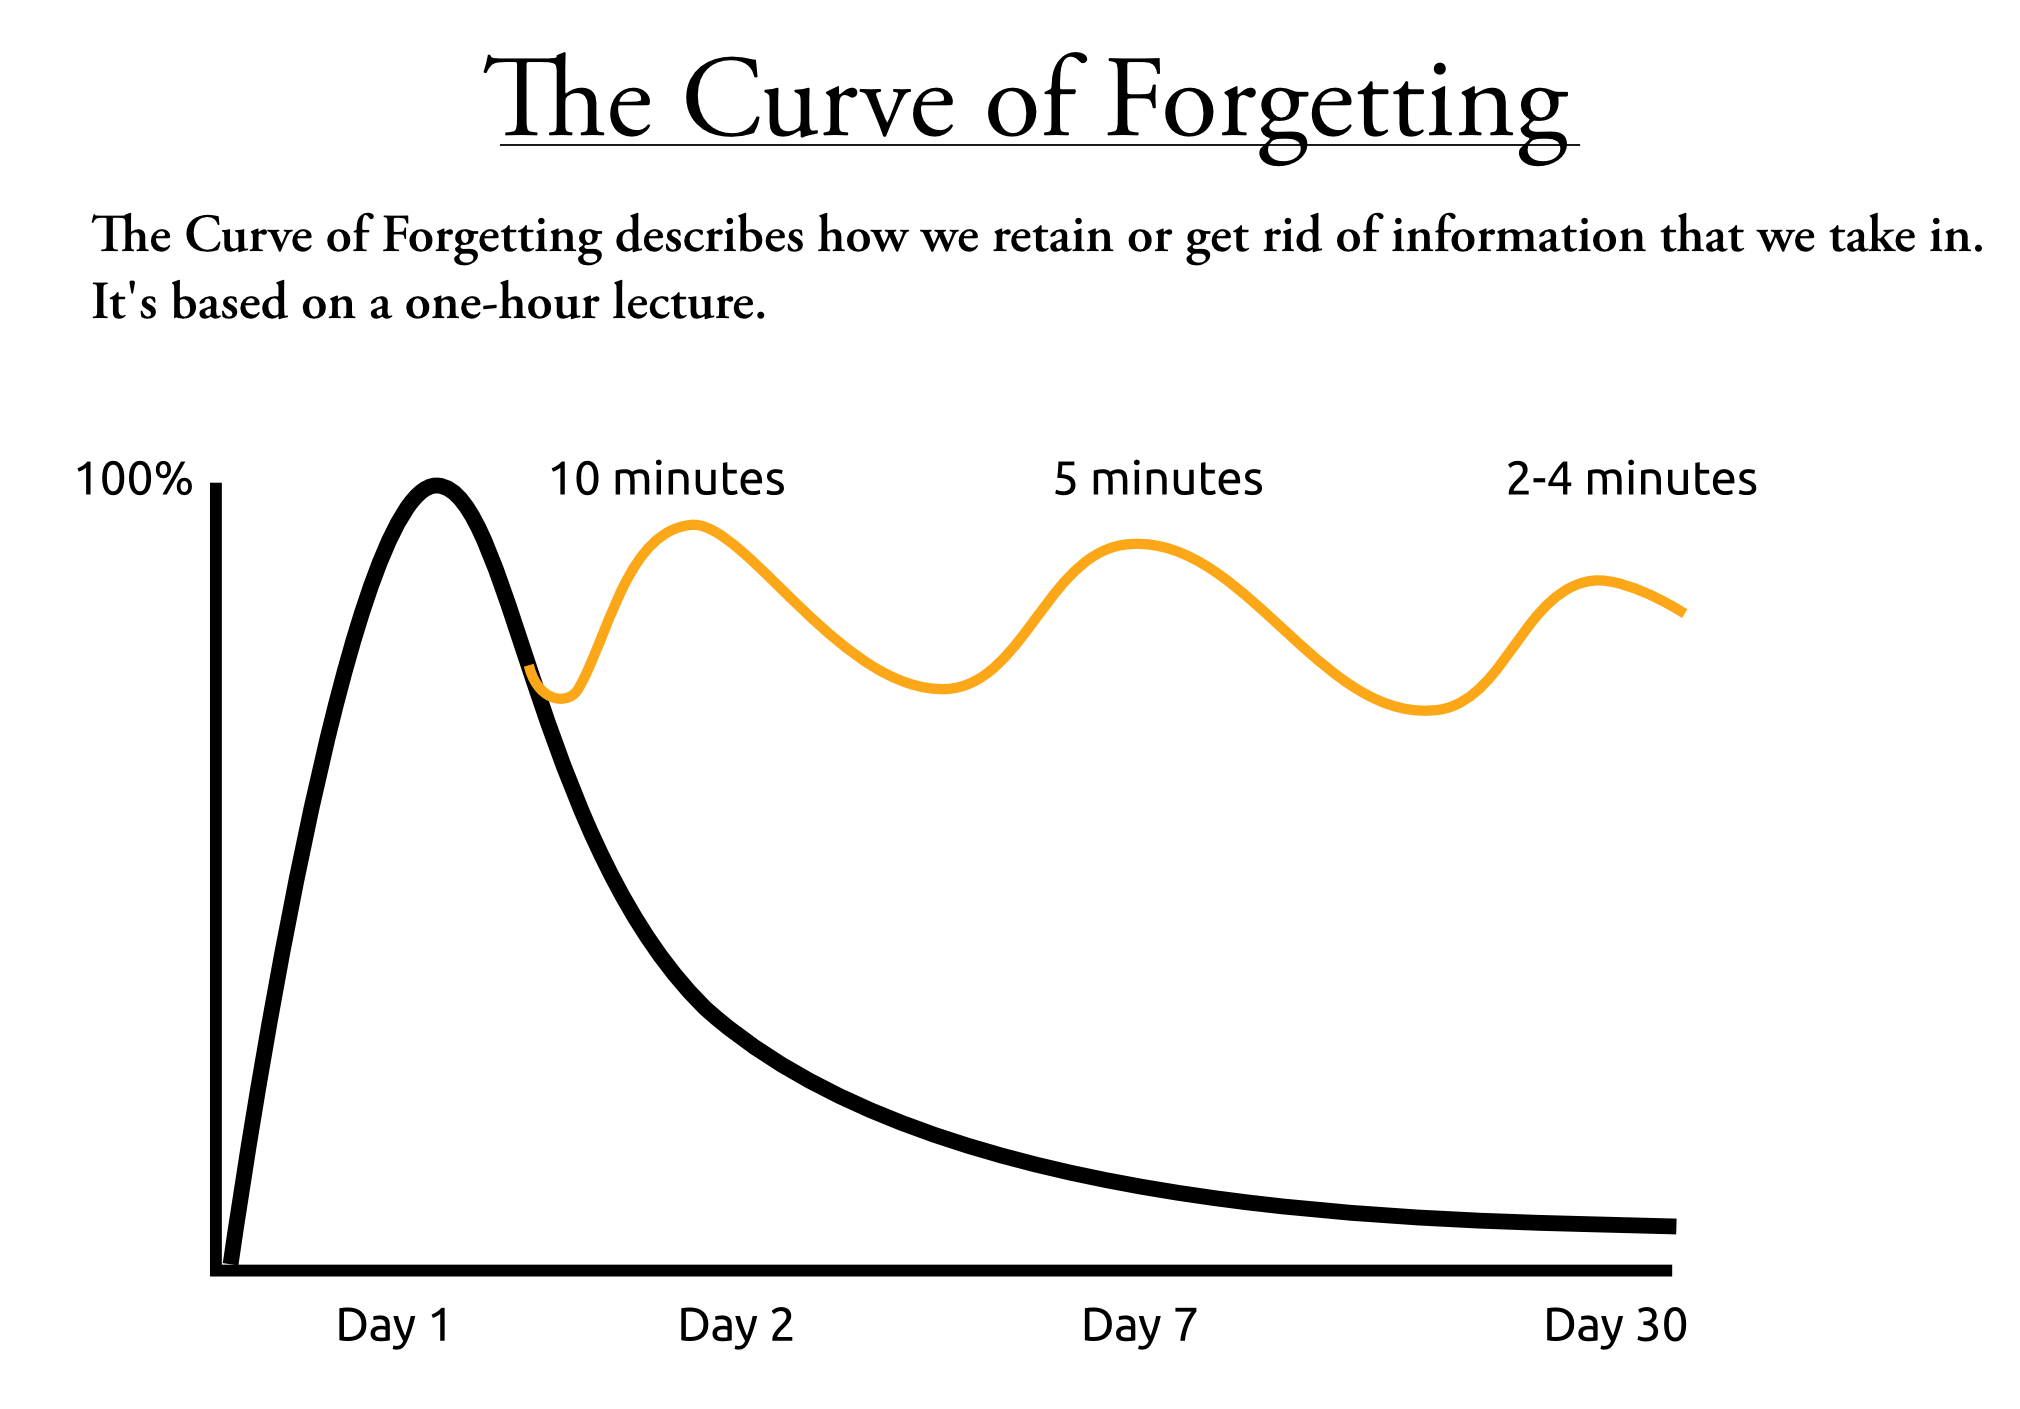
\includegraphics[width=0.8\textwidth]{forgeting-curve}
	\caption{forgeting-curve}
\end{figure}

No 1º dia, no início do estudo, você vai do ponto onde não sabe nada, ou 0\%, (onde a
curva começa na linha de base). No final do estudo você sabe 100\% do
que você estudou, onde a curva sobe para seu ponto mais alto.

No 2º dia, se você não fez nada com a informação que você aprendeu na
aula, não pensou sobre isso novamente, leu de novo, etc, você terá
perdido 50\% -80\% do que você aprendeu. Nossos cérebros estão
constantemente gravando informações em uma base temporária: pedaços de
conversas ouvidas na calçada, o que a pessoa na frente de você está
vestindo. Porque a informação não é necessária, e não vem de novo,
nossos cérebros descartam tudo isso, juntamente com o que foi aprendido
na estudo que você realmente deseja memorizar!

No 7 º dia, lembramos ainda menos, e no dia 30, mantemos cerca de 2\%
-3\% da hora original! Este bem coincide com os exames de meio do
bimestre, e pode ser responsável por nos fazer sentir como se nunca
tivéssemos visto aquilo antes.


É possível alterar a forma da curva! Reprocessando o mesmo bloco de
informações, enviando assim um grande sinal para o cérebro para
segurar esses dados. Quando a coisa se repete, seu cérebro diz: "Oh -
lá está ele de novo, é melhor eu manter isso." Quando você está
exposto à mesma informação várias vezes, leva-se menos e menos tempo
para "ativar" a informação em sua memória de longo prazo, e torna-se
mais fácil para você recuperar as informações quando você precisar
delas.

Aqui está a fórmula e o motivo para arrumar tempo de rever seu
material de estudo: Dentro de 24h da absorção da informação gaste 10
minutos revendo e você subirá a curva de memorização para quase 100\%
novamente. Uma semana depois (sete dias), levará apenas 5 minutos para
``reativar'' a mesma informação, e novamente elevar a curva. Em 30 dias,
seu cérebro necessitará de algo entre 2 e 4 minutos para lhe retornar
resultados, ``Sim, Eu sei disso\dots''

Frequentemente os estudantes acham que não conseguirão achar tempo para uma
revisão diária em sua agenda - Eles encontram problemas em manter o
rítmo. Noentanto, esta revisão é um excelente investimento de tempo.
Se você não revisar, você necessitará de 40 a 50 minutos reaprendendo
cada hora de material mais tarde - você tem tanto tempo assim?

Estudar exastivamente raramente proporcionará a retenção de
informações na memória de longo prazo de maneira satisfatória,
tornando difícil a recuperação dessas informações quando form
necessárias.

Dependendo do ritmo do seu estudo, a recomendação geral é gastar
meia hora no final de cada dia, e 1.5 a 2 horas cada final de semana
em atividades de revisão. Talvez você tenha tempo apenas para revisar
4 ou 5 dias da semana, e a curva se mantem na metade. Ok, é bem melhor
do que 2 a 3\% de retenção se você não fizer revisão alguma.

Muitos estudantes ficam maravilhados com a diferença proporcionada pelas
revisões regulares e em o quanto bem eles entendem e reteem materiais.
Vale a pena experimentar por algumas semanas, apenas pra ver a diferença
que isso fará para você!.

% subsection a_curva_de_esquecimento (end)

\subsection{Programas para memorização}
\label{sub:programas_para_memoria_o}

\noindent
Um excelente programa para trabalhar a memorização dentro dos intervalos
ideais de revisão chama-se \emph{Anki} o mesmo pode ser baixado para
Windows, Linux, Mac ou Android neste link \href{http://ankisrs.net/}{http://ankisrs.net/},
sua utilização é simples contudo segue também um link de um vídeo
sobre sua utilização básica \href{http://goo.gl/ueyFv}{http://goo.gl/ueyFv}

\vspace{0.3cm} \noindent {\footnotesize \ding{42} Leia um exceptional
artigo sobre o anki
\href{http://www.davidmansaray.com/anki-srs}{http://www.davidmansaray.com/anki-srs}
} \vspace{0.5\baselineskip}

\noindent
{\footnotesize \ding{42} If you are not willing to learn, no one can help you. If you are
determined to learn, no one can stop you. }
\vspace{0.3\baselineskip}

\noindent
Existe uma técnica de memorização chamada \href{http://goo.gl/Y5pRj}{repetição espaçada}
que consiste em repetir um pequeno trecho em intervalos regulares ao invés de
concentrar-se em uma seção longa de estudo, segundo estudos este
método é mais efetivo para memorização. De fato faz muito sentido, já
que quando estudamos por um longo período sem descanso nosso poder
de concentração diminuir. Outro fator é que o cérebro funciona de tal
forma que quando algo e visto mais de uma vez ele tende a reter, como
se ele ``pensasse assim'': Eu já vi isso uma vez, é melhor eu guardar
essa informação, neste caso ele guarda na nossa memória de longo prazo.

\vspace{0.3\baselineskip}
\noindent
Você pode recortar uma cartolina formando os cartões e preenche-los
de um lado com uma frase em inglês e do outro com sua tradução,
utilize cores para tornar os cartões mais atraentes.


\newpage
\begin{figure}[h!]
	\centering
	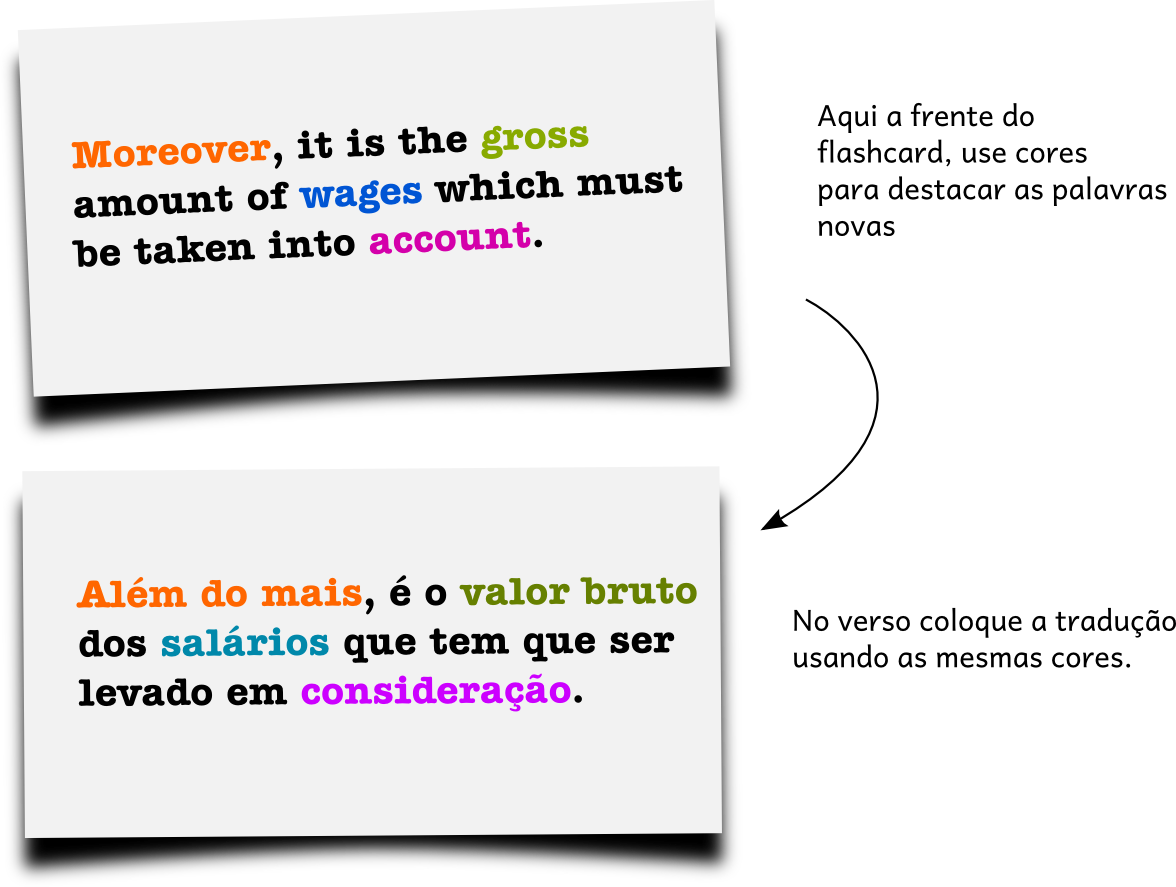
\includegraphics[width=0.8\textwidth]{flashcard}
	\caption{flashcard}
\end{figure}

% subsection programas_para_memoria_o (end)


\subsection{A pirâmide do aprendizado}
\label{sub:a_pir_mide_do_aprendizado}

Outro aspecto a ser considerado acerca da memoriação é quão eficientes
somos em gravar a informação inicial, ou seja, não adiantam muitas
técnicas de momorização para o que não foi sequer absorvido, é aí que
entra a \emph{Pirâmide do aprendizado}, que nos mostra através de pesquisas
feitas pela Universidade de Queens em Belfast, dados sobre quais são
os métodos de estudo mais eficientes para reter a informação inicial.
Ou seja, quais métodos geram uma melhor impressão em nossos cérebros.

\begin{figure}[ht!]
	\centering
	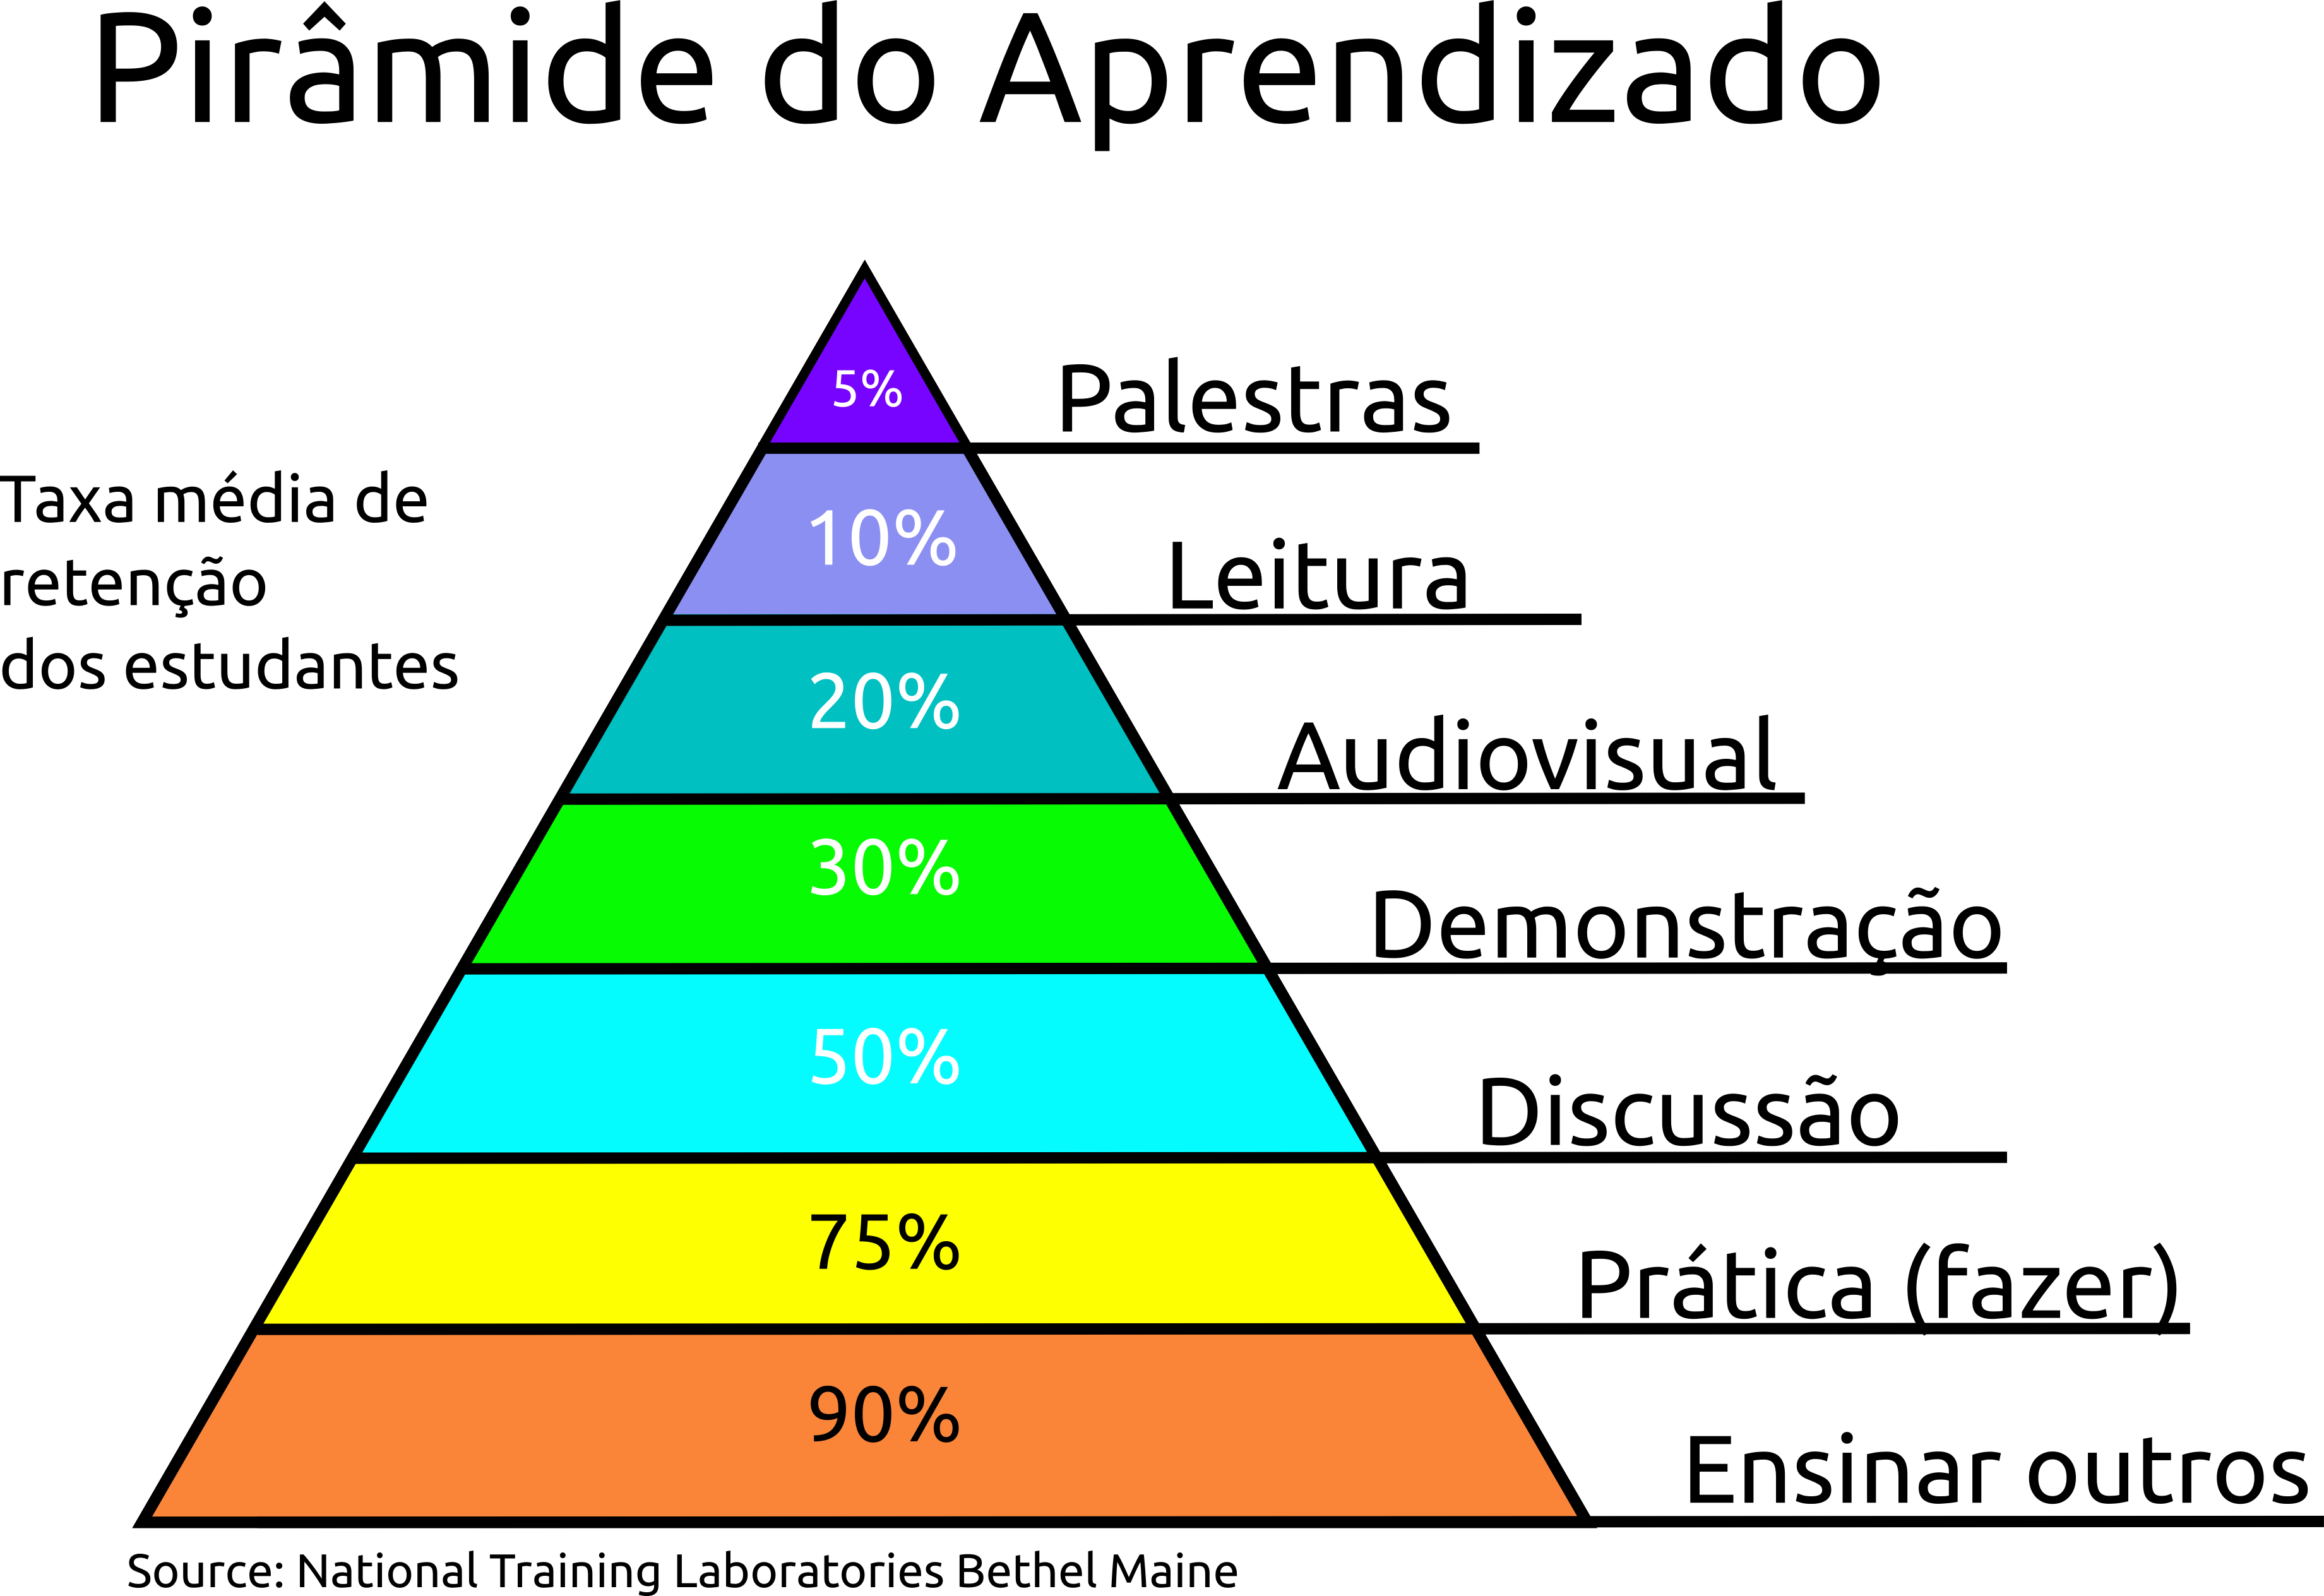
\includegraphics[width=0.6\textwidth]{piramide-do-aprendizado}
	\caption{piramide-do-aprendido}
\end{figure}

\newpage
O modelo proposto pela \emph{Pirâmide do aprendizado} está sendo
questionado por muita gente na internet basicamente com a seguinte
argumentação, se uma palestra for feita por alguém bem preparado
gerará mais retenção de aprendizado do que o ato de ensinar feito
por alguém menos preparado, ou coisa do tipo, mas na verdade a
proposta da pirâmide se resume a:

\begin{description}
	\item [ação] Os estudantes devem ser expostos a métodos de aprendizado ativos, isto significa que uma
		palestra que em geral tem baixo nível de retenção, caso envolva
		emocionalmente a plateia, caso crie interações com a mesma, elevará o
		seu nível de retenção. Isso explica o fato de que boas
		palestras geram mais retenção.
	\item [solução de problemas] O conhecimento deve ser absorvido através de compartilhamento e solução de problemas
	\item [pensar] Os estudantes devem, analizar sintetizar e avaliar
\end{description}

% subsection a_pir_mide_do_aprendizado (end)

\subsection{Aprendizado consciente e acidental}
\label{sub:aprendizado_consciente_e_acidental}

Durante sua jornada de aprendizado procure equilibrar a quantidade
de tempo dedicado ao estudo consciente e ao estudo casual, a diferença
entre ambos é descrita abaixo de forma simples.

\begin{description}

	\item[Aprendizado deliberado ou consciente] Acontece quando você
		etuda inglês, talvez você sublinhe palavras que você não
		conhece em um jornal, artigo ou em um livro, então abre o
		dicionário, cria flashcards (leia sobre o anki na
		página~\pageref{sub:programas_para_memoria_o}), estude
		gramática etc. Você ativamente tenta aprender e lembrar
		inglês.

	\item[Aprendizado acidental] Acontece quando você não está
		tentando aprender, ou memorizar nada - você está apenas se
		divertindo. Por exemplo: enquando você ouve um podcast, lê um
		livro e ... uma palavra ou frase salta em sua frente. Talvez
		você venha tentando lembrar aquela palavra antes e não
		conseguiu memoriza-la ainda, mas desta vez o contexto ajuda
		você de tal forma que vem aquele estalo na mente "Ah-Há!".
		Neste momento você não mais irá esquecer aquela palavra, isto
		é o aprendizado acidental.

\end{description}

Quando você deliberadamente tenta aprender uma palavra você a coloca
em sua memória, quando você escuta uma palavra acidentalmente você cria
um link entre a palavra na memória e a mesma palavra no contexto e a
fixa em seu cérebro.

Tente criar a maior número de oportunidades para o aprendizado
acidental possível, seja colocando filmes com som inglês e legenda em
português e vice-versa, seja ouvindo podcasts na fila do banco etc. No
futuro, quando você tiver um bom vocabulário, uma boa forma de unir o
aprendizado acidental com o consciente é estudar inglês ouvindo um
falante nativo do inglês lhe ensinando inglês, mas lembre-se que para
isso você deve ler o livro das \emph{1000 palavras mais comuns do
ingês}\footnote{http://goo.gl/jbyBZ} citado anteriormente, em minha
experiência pessoal este livro foi fundamental e o será também para
você!

\vspace{0.3\baselineskip}
\noindent
{\footnotesize \ding{42} Muitas pessoas acabam focando por demais em um dos dois métodos,
sendo que o ideal o balanceamento entre os dois, tanto deliberado como
casual}.


% subsection aprendizado_consciente_e_acidental (end)

\newpage
\subsection{Interação}\label{sub:interacao}

O professor americano \index{H.J Hoge} ``H.G Hoge'' criou o método \index{H.J
Hoge!Effortless English}
\href{http://www.effortlessenglishpage.com/p/7-rules.html}{``Effortless
English''}\footnote{Inglês sem esforço:
http://www.effortlessenglishpage.com/p/7-rules.html} ou  Inglês sem Esforço
-- para saber mais acesse este endereço:
\href{http://goo.gl/DyfZ7}{http://goo.gl/DyfZ7} -- basicamente este método usa
mini-histórias com as quais o ouvinte tem que interagir, a história é contada
e em seguida, frase por frase, são feitas várias perguntas na qual você deve
dar respostas. O conteúdo da história é bem simples para que as respostas seja
automáticas o usuário deve repetir a audição da mini história durante uma ou
duas semanas a fim de conseguir o que o professor ``HG Hoge'' chama de ``Deep
Learning'' ou aprendizado profundo no qual o estudante não tem sequer que pensar
nas respostas, as mesmas surgem naturalmente, o método é fortemente baseado na
repetição. Aqui um link
\href{http://goo.gl/ECXTr}{http://goo.gl/ECXTr}
do torrent\footnote{Protocolo de rede para permitir downloads mais rápidos}
para o curso, em que você terá que baixar um arquivo tar.bz2, descompactar e só
então terá o torrent. {\footnotesize \ding{42} É possível que ele exiba uma
janela ``pop-up.''}

Na verdade, o sistema {\em Effortless English} foi projetado com base em várias
pesquisas feitas pelos maiores especialistas e doutores em aprendizagem de idiomas no
mundo: Stephen Krashen, James Asher, J. Marvin Brown, Ashley Hastings, Brenda Murphy, David Long e Blaine Ray.

\vspace{0.3\baselineskip} \noindent {\footnotesize \ding{42}
``\dots Formular regras e ensinar fatores complexos sobre a lingua alvo
não é ensino de línguas, mas ao contrário é `apreciação da língua' ou linguística.''
\href{http://www.readability.com/articles/ndsyiy1q}{{\em Stephen Krashen}}}

\vspace{0.3\baselineskip} \noindent {\footnotesize \ding{42} ``Acquisition requires
meaningful interaction in the target language - natural communication - in
which speakers are concerned not with the form of their utterances but with
the messages they are conveying and understanding.''
\href{http://www.readability.com/articles/ndsyiy1q}{{\em Stephen Krashen}}}

\vspace{0.3\baselineskip} \noindent {\footnotesize \ding{42} ``In the real world,
conversations with sympathetic native speakers who are willing to help the
acquirer understand are very helpful.''
\href{http://www.readability.com/articles/ndsyiy1q}{{\em Stephen Krashen}}}

\begin{figure}[h!]
	\centering
	\caption{Dr Stephen Krashen em uma palestra}
	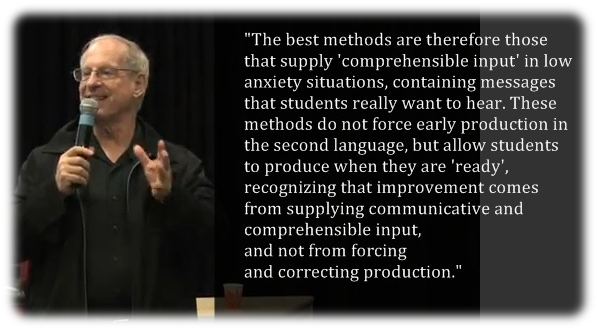
\includegraphics[width=0.8\textwidth]{input}
\end{figure}

\vspace{0.3\baselineskip}
\noindent
``Os melhores métodos são portanto os que fornecem `entrada compreensível'
em situações de baixa ansiedade, contendo mensagens que os estudantes realmente
querem ouvir. Estes métodos não forçam a produção precoce em uma segunda linguagem, mas
permitem aos estudantes produzir quando eles estiverem prontos, reconhecendo
que a melhora vem pelo suprimento de mensagens inteligíveis, e não forçando e
corrigindo o que foi produzido.'' {\em Stephen Krashen}


\newpage
%\vspace{-1.2cm}
\section{Como usar o google para aprender inglês}\label{sec:google}
\index{google}

\noindent Para o navegador firefox instale a extensão gtranslate
\href{http://goo.gl/RQbt4}{http://goo.gl/RQbt4} você instala a extensão
clicando no botão verde, seleciona uma palavra para mostrar a tradução.
Após instalada a extensão você seleciona um texto em uma página web e clica com o botão
direito como visto na figura abaixo

\begin{figure}[h!]
	\centering
	\caption{\footnotesize Firefox gtranslate addon}
	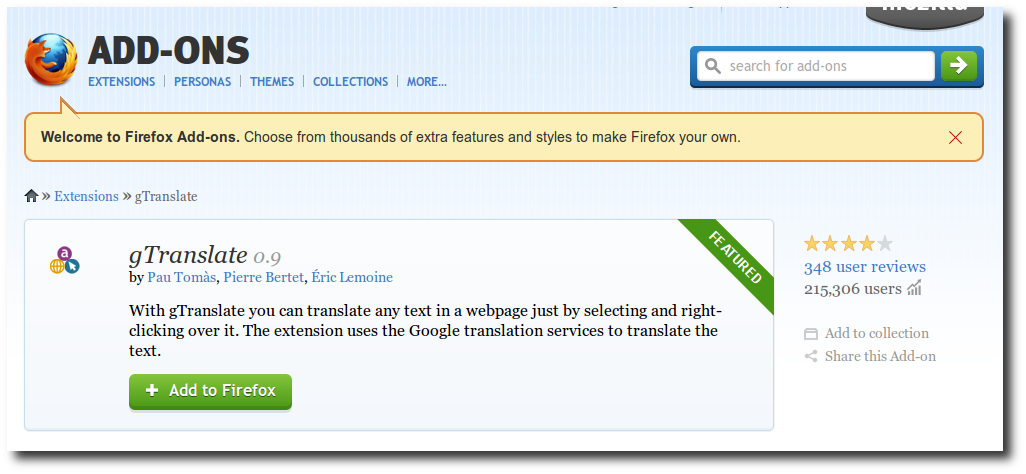
\includegraphics[width=0.8\textwidth]{gtranslate1}
	\index{Firefox!granslate}
\end{figure}

\begin{figure}[h!]
	\centering
	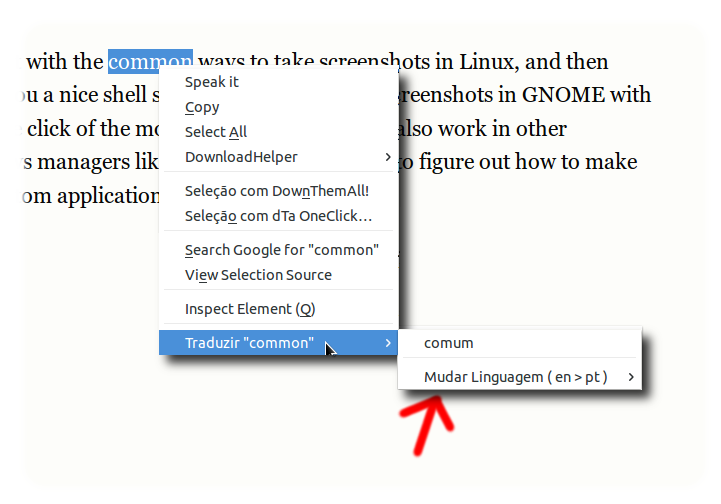
\includegraphics[width=0.8\textwidth]{gtranslate-menu}
\end{figure}

\begin{center}
\noindent
{\footnotesize \ding{42} lembre-se de selecionar o idioma no local indicado.}
\end{center}

\noindent
{\footnotesize \ding{42} Lembre-se que os recursos que mostraremos a seguir só serão melhor aproveitados
se você obtiver um resultado no qual a palavra buscada esteja em um contexto.}

\vspace{0.3\baselineskip}
\noindent
{\footnotesize \ding{42} Na página~\pageref{img:video-helper}, seção \ref{sec:ouca}
descubra como baixar vídeos do youtube}

\newpage
\noindent
Se você digitar no google {\em What does {\bf dig} mean}, ele retornará \dots

\begin{figure}[h!]
	\centering
	\caption {O significado de {\bf dig}}
	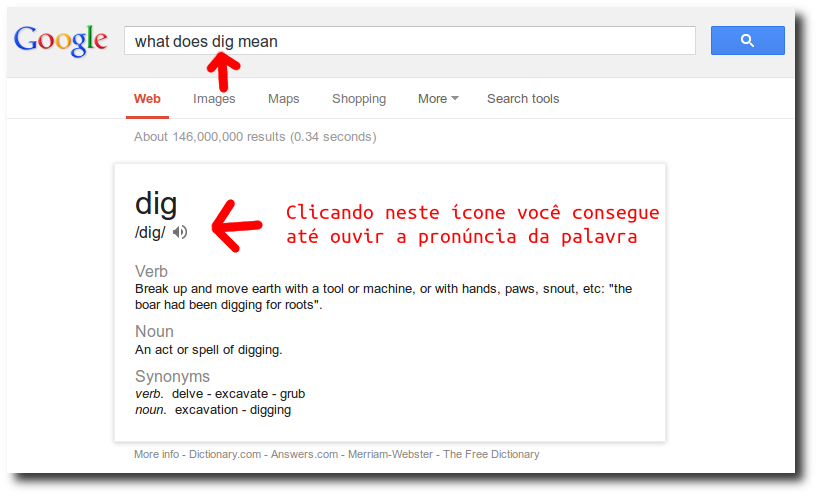
\includegraphics[width=0.8\textwidth]{google}
\end{figure}

\begin{figure}[h!]
	\centering
	\caption{Usando o google tradutor}
	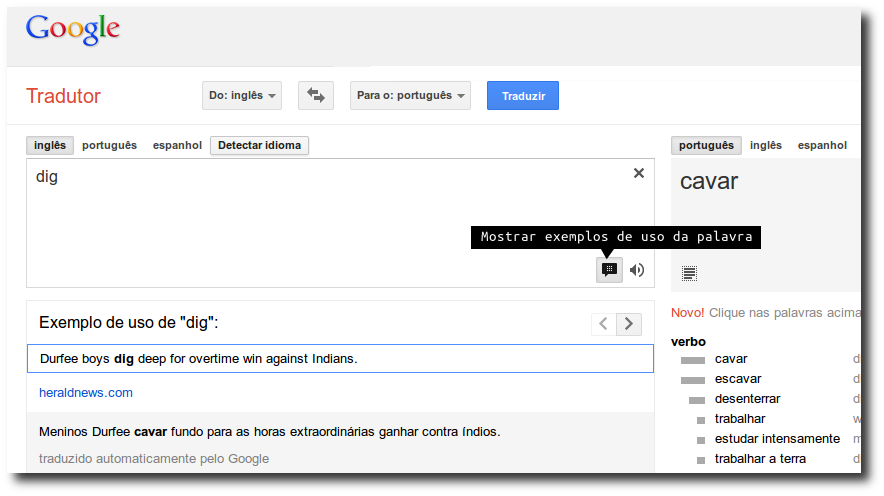
\includegraphics[width=0.8\textwidth]{google-translate}
\end{figure}

\noindent
Na janela do google translate você pode clicar no auto-falante para ouvir
o som em cada idioma bem como clicando sobre a palavra traduzida ele lhe
dá um exemplo contextualizado, clicando sobre o contexto dado ele exibe
a tradução da frase contextualizada.

Do mesmo modo que você pode estudar a gramática de um idioma simplesmente
convivendo com o mesmo, pode também estudar inglês sem pensar diretamente em
estudar inglês, muitas crianças aprendem muitas palavras em inglês simplesmente
porque elas estão presentes nos seus video games.

\section{Como tornar páginas na web mais legíveis}
\index{Firefox!Legibilidade}

Durante seu estudo do inglês você por vezes vai se deparar com um problema
bastante comum, o layout\footnote{a disposição dos caracteres na tela e seu
tamanho na tela} na maioria das vezes dificulta a leitura, neste ponto você está se
deparando com um problema bem diverso do seu foco que é melhorar
seu inglês, o texto está lá, mas a sua legibilidade
está prejudicada, a fim de contornar este problema instale a extensão readability a mesma
pode ser encontrada neste link \href{http://www.readability.com/addons}{http://www.readability.com/addons}.

\begin{figure}[h!]
	\centering
	\caption{{\footnotesize Clique no botão verde}}
	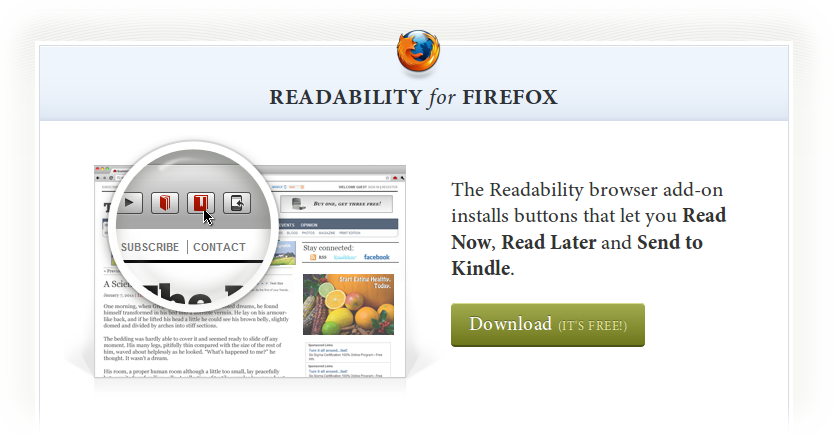
\includegraphics[width=0.8\textwidth]{readability-1}
\end{figure}

\begin{figure}[h!]
	\centering
	\caption{{\footnotesize Texto transformado com o readability}}
	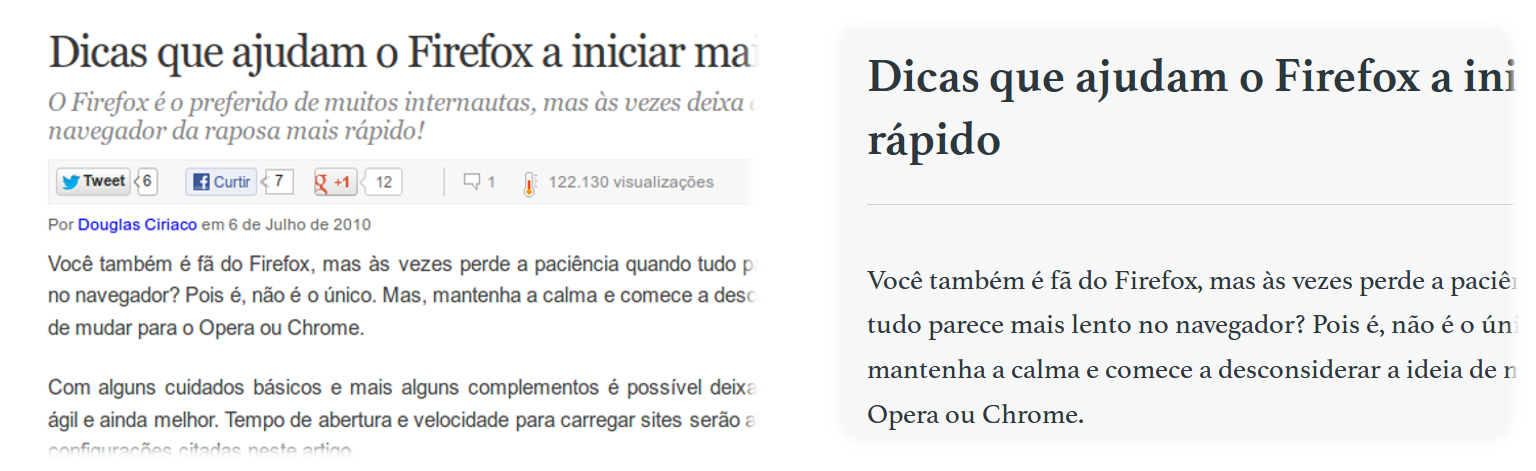
\includegraphics[width=1.2\textwidth]{readability-2}
\end{figure}

\begin{center}
{\footnotesize \ding{42}
Leia sobre o readability aqui: \href{http://tecnoblog.net/35554/ler-texto-sites-como-ebook-reader/}{http://goo.gl/a51mu}\footnote{http://tecnoblog.net/35554/ler-texto-sites-como-ebook-reader/}}
\end{center}


